%! TeX root = ../main-zh.tex
% 封底（中英文两版共用版式，文字在 style/lang-zh.tex、style/lang-en.tex 的 \BackCover... 里）。
% 版式和封面（frontmatter/cover.tex）呼应：
%   上半部白底：只有“关于作者”，旁边贴着那张小小的猫狗大战；
%   下面一条深红色的横带，横带下面是封面上那张彩色照片，一直铺到页面底边；
%   左下角是“出版社”的标志。
% 封底必须是偶数页（翻过来就是书的背面），不是的话先空一页。

\clearpage
\ifodd\value{page}\null\thispagestyle{empty}\clearpage\fi
\thispagestyle{empty}

\definecolor{coverred}{RGB}{190,30,45}
\definecolor{covergray}{RGB}{90,90,90}
\newfontfamily\backcoverfont{texgyrepagella}[
  Extension=.otf, Ligatures=TeX, UprightFont=*-regular, BoldFont=*-bold,
  ItalicFont=*-italic, BoldItalicFont=*-bolditalic]

\begin{tikzpicture}[remember picture, overlay, every node/.style={inner sep=0pt}]
  \coordinate (TL) at (current page.north west);

  % ---- 下半部：彩色照片，从横带的下沿一直铺到页面底边 ----
  \begin{scope}
    \clip ($(TL) + (0,-200mm)$) rectangle (current page.south east);
    \node[anchor=south] at (current page.south)
      {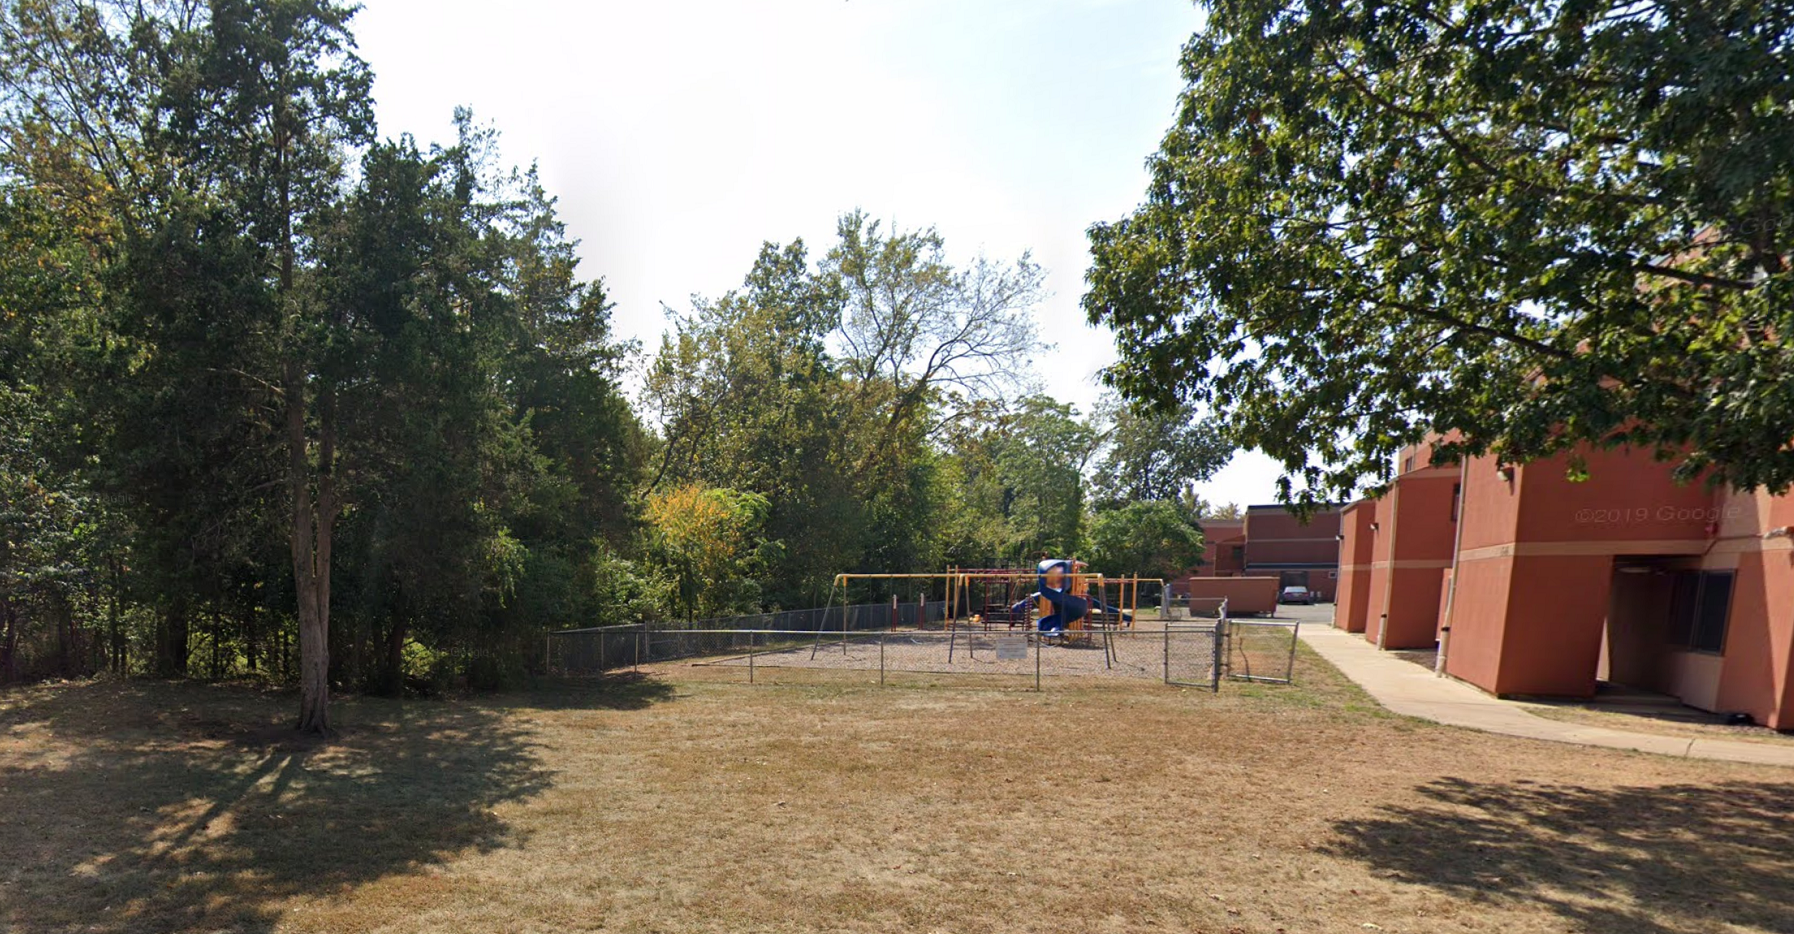
\includegraphics[width=\paperwidth]{figures/cover.png}};
  \end{scope}

  % ---- 深红色的横带（页面顶端往下 192--200 mm）----
  \shade[left color=coverred, right color=coverred!85!black, opacity=0.94]
    ($(TL) + (0,-192mm)$) rectangle ($(current page.north east) + (0,-200mm)$);

  % ---- 上半部：关于作者 ----
  \node[anchor=north west, text width=112mm, align=justify, text=black!80,
        font=\backcoverfont\fontsize{12}{19}\selectfont]
    (bio) at ($(TL) + (24mm,-122mm)$)
    {{\lazyfont\bfseries\large\color{coverred}\BackCoverAuthorTitle}\par\medskip\BackCoverAuthor};

  % ---- 作者旁边：小小的猫狗大战（原图 1204×772 像素，trim 裁掉底部的水印和 START 按钮）----
  \node[anchor=north east, rotate=4, fill=white, inner sep=1.5mm,
        drop shadow={opacity=0.4, shadow xshift=0.8mm, shadow yshift=-0.8mm}]
    at ($(bio.north east) + (49mm,1mm)$)
    {
\includegraphics[trim=0 112 0 0, clip, width=40mm]{figures/catdog.png}};

  % ---- 左下角：“出版社”的标志（和封面一样）----
  \fill[white, opacity=0.88] ($(current page.south west) + (14mm,14mm)$) rectangle ++(31mm,19mm);
  \node[text=coverred, font=\backcoverfont\bfseries\fontsize{30}{30}\selectfont]
    at ($(current page.south west) + (24mm,26mm)$) {C};
  \node[text=covergray, font=\backcoverfont\fontsize{19}{19}\selectfont]
    at ($(current page.south west) + (35.5mm,26.5mm)$) {\{\,\}};
  \node[text=covergray, font=\backcoverfont\fontsize{6.5}{8}\selectfont\addfontfeature{LetterSpace=10}]
    at ($(current page.south west) + (29.5mm,17.8mm)$) {LAZY PRESS};
\end{tikzpicture}
